\documentclass[assd_tp2_main.tex]{subfiles}

\begin{document}

\section{Efectos de audio}

\subsection{Reverbebrador}

\subsubsection{Implementación de eco simple}

Se implemento un eco simple utilizando el sistema

\begin{equation}
	y(n)=x(n)+gx(n-M)
\end{equation}

Se muestran a continuación los resultados con una señal de prueba

\begin{figure}[H]	
	\centering
	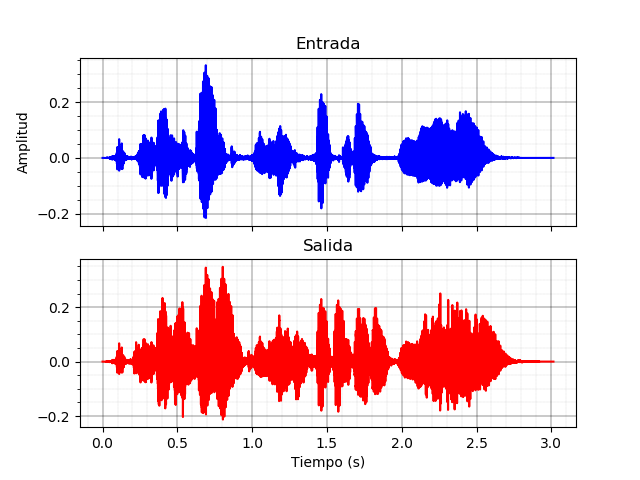
\includegraphics[scale=1]{graficos/EJ8/eco_simple.png}
	\caption{Resultados con $M=5000$, $g=0.999$ }
	\label{fig:bloqueElemental}
\end{figure}

Se puede observar de los resultados intuitivamente como la señal de salida contiene repeticiones de la señal de entrada, y al escuchar el audio se pudo notar dicho efecto de eco. Fue necesario colocar un retraso muy grande ($M=5000$) y una ganancia muy alta ($g=0.999$) para que el efecto fuera notorio

\subsubsection{Implementación de reverberación plana}
Se implementó una reverberación plana utilizando una ecuación de diferencias con feedback. 
\begin{equation}
	y(n)=x(n)+gy(n-M)
\end{equation}
Se muestran a continuación los resultados con una señal de prueba
\begin{figure}[H]	
	\centering
	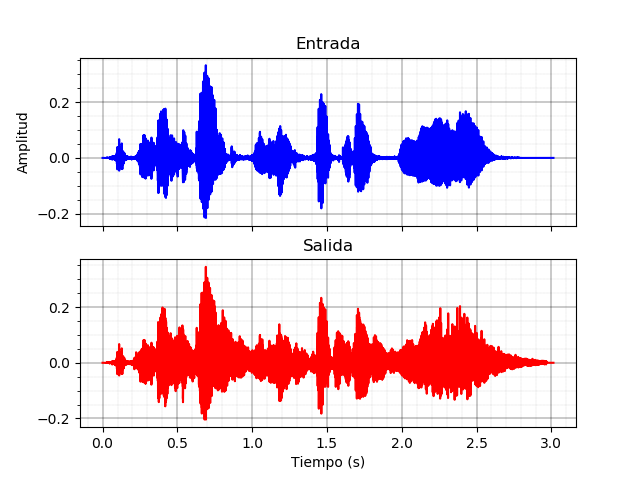
\includegraphics[scale=1]{graficos/EJ8/eco_plano.png}
	\caption{Resultados con $M=500$, $g=0.5$ }
	\label{fig:bloqueElemental}
\end{figure}
Se necesitó disminuir fuertemente el valor de $g$ para evitar que la salida saturara. Al tener realimentación (es decir, ser IIR) el sistema puede perder la estabilidad con facilidad

\subsubsection{Implementación de reverberación pasa bajos}


\end{document}

